\documentclass[hyperref={colorlinks,citecolor=blue,linkcolor=blue,urlcolor=blue}]{beamer}

\mode<presentation>
{
  \usetheme{Madrid}       % or try default, Darmstadt, Warsaw, ...
  \usecolortheme{default} % or try albatross, beaver, crane, ...
%   \usefonttheme{serif}    % or try default, structurebold, ...
  \setbeamertemplate{navigation symbols}{}
  \setbeamertemplate{caption}[numbered]
  \setbeamertemplate{frametitle}[default][center]
} 

\usepackage[english]{babel}
\usepackage[utf8x]{inputenc}
\usepackage{transparent}
\usepackage{subcaption}
\usepackage{caption}
\usepackage{setspace}
\usepackage{amsmath}
\usepackage{amssymb}
\usepackage{chemfig}
\usepackage[version=3]{mhchem}
\sffamily
% Here's where the presentation starts, with the info for the title slide
\title{Towards Learning Better and Flexible Representations from Variational Autoencoders}
\author{Advait, Pulkit, Sanchit}
\institute{IIT Bombay}
\date{20th April 2024}

\begin{document}

\begin{frame}
  \titlepage
\end{frame}

% These three lines create an automatically generated table of contents.
\begin{frame}{Outline}
  % \doublespacing
  \tableofcontents
  \singlespacing
\end{frame}

\section{Representation Learning}

\begin{frame}{\transparent{0.4} Towards \transparent{1}\textbf{Learning} \transparent{0.4}Better and Flexible \transparent{1}\textbf{Representations} \transparent{0.4}from Variational Autoencoders\transparent{1} \vspace{0.3em}}
\begin{itemize}
  \item Representation Learning is concerned with learning representations of the data that make it easier to extract useful information.
  \item The learned representations can then be used to perform multiple downstream tasks such as classification or retrieval.
  \vspace{1em}
  \pause
  \begin{figure}
    \captionsetup{oneside,margin={-1cm,0cm}}
    \begin{subfigure}[b]{0.3\textwidth}
        \centering
        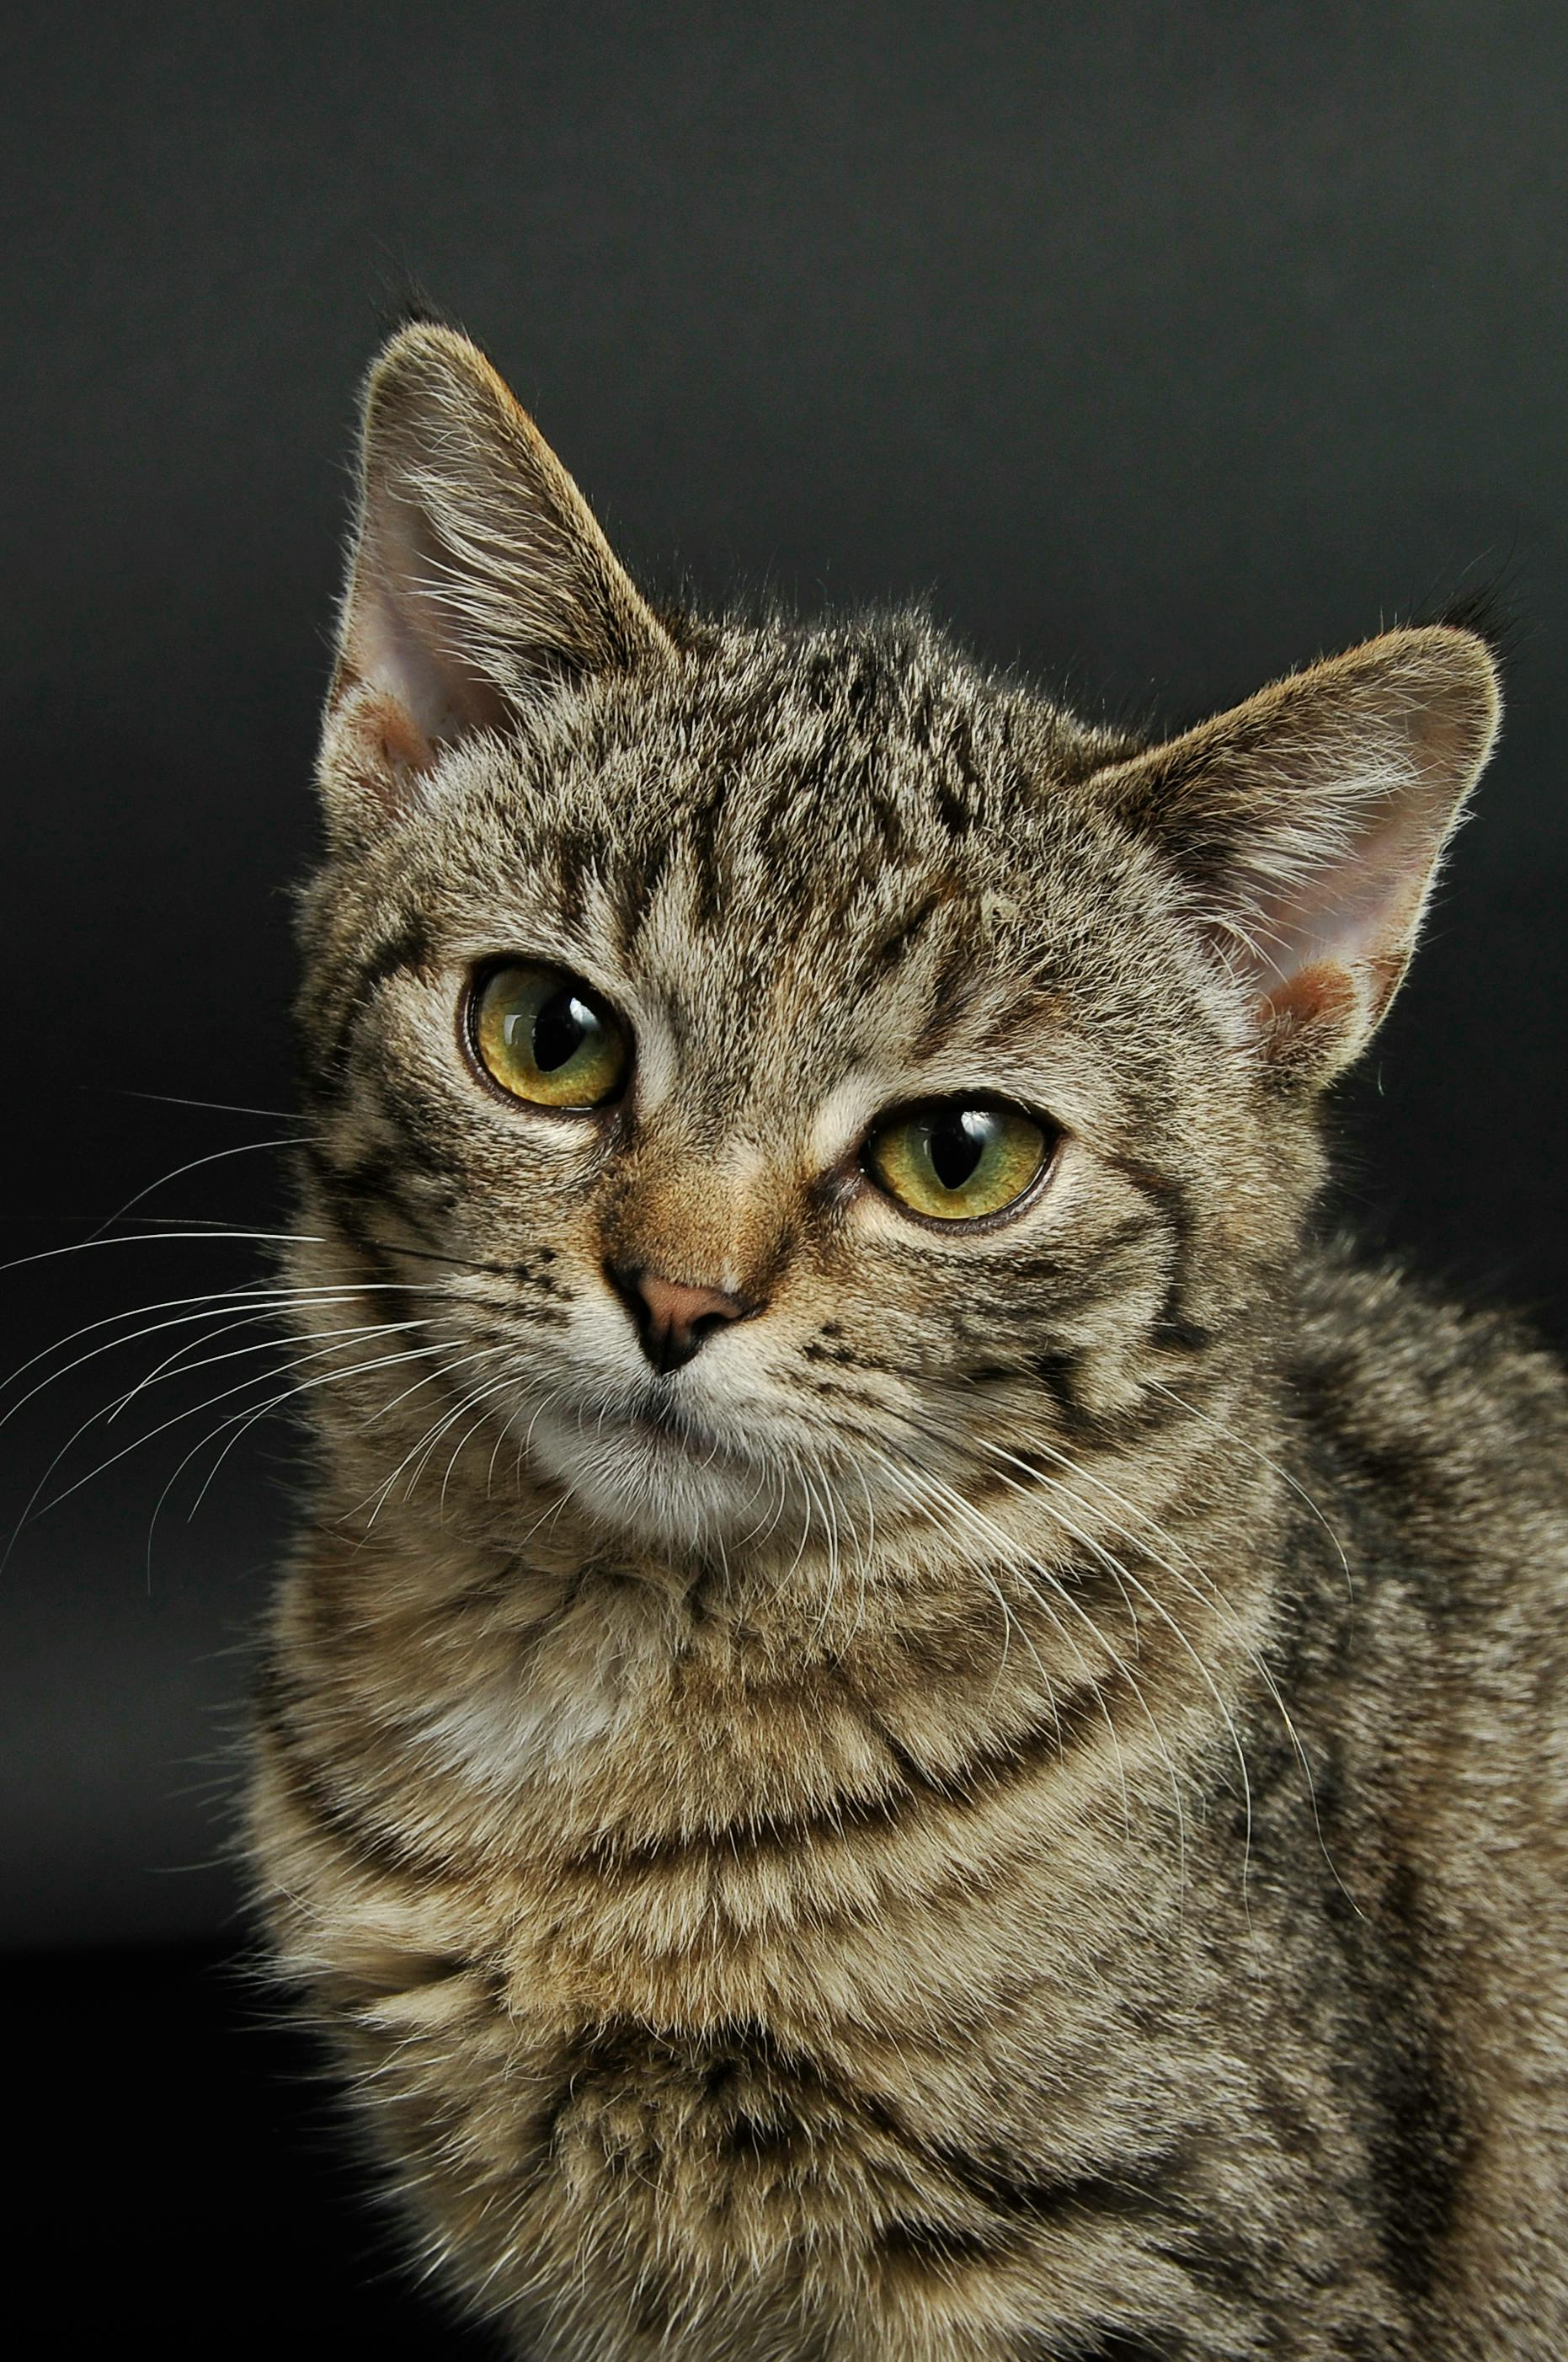
\includegraphics[width=0.6\textwidth,]{./Images/cat-image.jpeg}
    \end{subfigure}
    \pause
    \hspace{-2em}
    \begin{subfigure}[b]{0.3\textwidth}
        \centering
        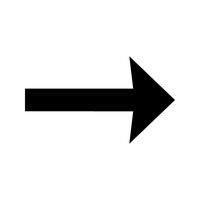
\includegraphics[width=0.8\textwidth]{./Images/arrow.jpeg}
    \end{subfigure}
    \hspace{-4em}
    \pause
    \begin{subfigure}[b]{0.3\textwidth}
        \centering
        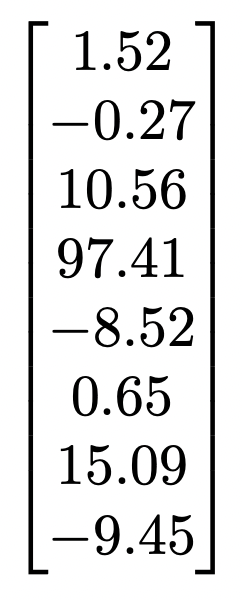
\includegraphics[width=0.35\textwidth]{./Images/column.png}
    \end{subfigure}
    \vspace{0.5em}
    \caption{Representating the image of cat as 8-dimensional vector}
  \end{figure}
\end{itemize}
\end{frame}

\begin{frame}{\transparent{0.4} Towards \transparent{1}\textbf{Learning} \transparent{0.4}Better and Flexible \transparent{1}\textbf{Representations} \transparent{0.4}from Variational Autoencoders\transparent{1} \vspace{0.3em}}
\begin{itemize}
  \item An ideal representation should be expressive, meaning that a reasonably-sized learned representation should capture a huge number of possible input configuration.
  \item Moreover, we expect the process of learning representations to not be computationally expensive.
  \item Some examples of models used for representation learning :-
  \begin{enumerate}
    \item Convolutional Neural Networks for Image Representations
    \item Recurrent Neural Networks or Transformers for Word Representations
  \end{enumerate}
  \item In this project, we focus our attention on learning representations of images using \textbf{Variational Autoencoders}
\end{itemize}
\end{frame}

\section{Representation Learning using VAEs}
\subsection{Intro to Variational Autoencoder}

\begin{frame}{\transparent{0.4} Towards Learning Better and Flexible Representations from \transparent{1} \textbf{Variational Autoencoders} \vspace{0.3em}}
  \begin{itemize}
    \item Variational autoencoders (VAEs) are a deep learning technique for learning latent representations.
    \item VAEs consist of an encoder network which models the posterior distribution $q_{\phi}(\mathbf{z} | \mathbf{x})$ and a decoder network which models the likelihood distribution $p_{\theta}(\mathbf{x} | \mathbf{z})$
    \item VAEs have been used for several applications such as dimensionality reduction and image generation.
  \end{itemize}
  \vspace{0.5em}
  \pause
  \begin{center}
    \begin{figure}
      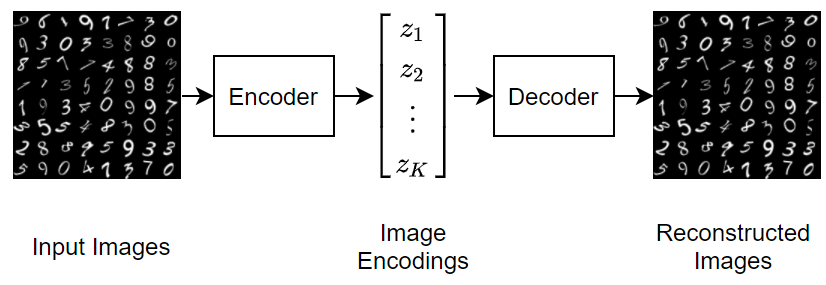
\includegraphics[width=0.7\textwidth]{./Images/vae.png}
      \caption{Variational Autoencoder Architecture}
    \end{figure}
  \end{center}
\end{frame}

\subsection{Experimental Setup}

\begin{frame}{\transparent{0.4} Towards \transparent{1}\textbf{Learning} \transparent{0.4}Better and Flexible \transparent{1}\textbf{Representations from Variational Autoencoders} \vspace{0.3em}}
  \begin{itemize}
    \item After training the VAE on the ELBO objective, the learned  $q_{\phi}(\mathbf{z} | \mathbf{x})$ can be used to generate the representation.
    \item For of a given data $\mathbf{x'}$, we can obtain a representation by :- 
    \begin{enumerate}
      \item Sampling from the posterior - $\mathbf{z'} \sim q_{\phi}(\mathbf{z} | \mathbf{x'})$
      \item Finding the most likely representation (MAP) - $\mathbf{z'} = \text{argmax} \; q_{\phi}(\mathbf{z} | \mathbf{x'})$
    \end{enumerate}  
    \item For this project, we used two popular image datasets :-
    \begin{figure}
      \pause
      \begin{subfigure}[b]{0.4\textwidth}
          \centering
          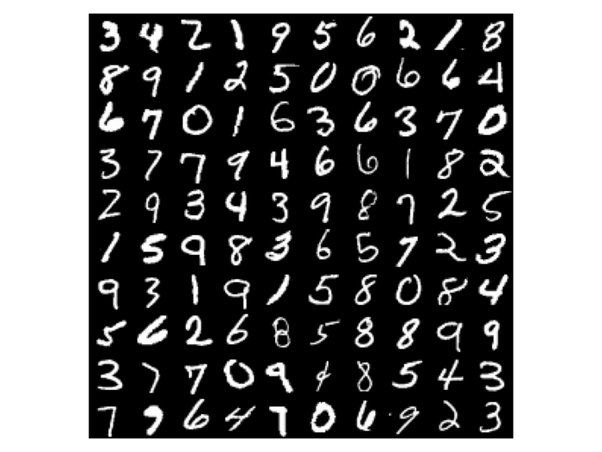
\includegraphics[width=0.95\textwidth,]{./Images/mnist.jpeg}
          \caption{MNIST Dataset}
      \end{subfigure}
      \pause
      \begin{subfigure}[b]{0.4\textwidth}
          \centering
          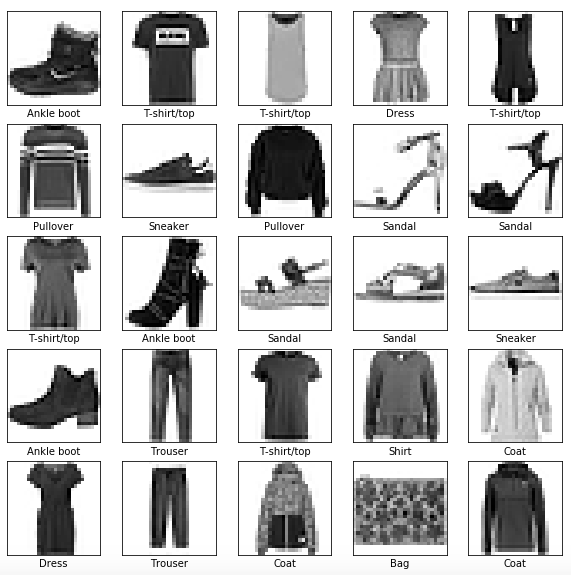
\includegraphics[width=0.7\textwidth]{./Images/FashionMNIST.png}
          \caption{FashionMNIST Dataset}
      \end{subfigure}
    \end{figure}
  \end{itemize}
\end{frame}

\begin{frame}{\transparent{0.4} Towards \transparent{1}\textbf{Learning} \transparent{0.4}Better and Flexible \transparent{1}\textbf{Representations from Variational Autoencoders} \vspace{0.3em}}
  \begin{itemize}
    \item For the downstream classification task, we used a feedforward Network consisting of 2 linear layers.
    \item The encoder and decoder networks of VAE consist of 2 convolutional layers and 2 linear layers.
    \item The classifier and VAE have been implemented in PyTorch and we have used Adam Optimizer for training the models.
    \item We varied the size of latent representations as [2, 8, 16, 32, 64, 128].
    \item VAE was trained for 10 epochs with a batch size of 32 meanwhile the classifier was trained for 20 epochs.
    \item We implemented an early stopping module to prevent overfitting.
    \item For evaluation, we have employed 5-fold cross validation.
  \end{itemize}
\end{frame}

\subsection{Results}

\begin{frame}{\transparent{0.4} Towards \transparent{1}\textbf{Learning} \transparent{0.4}Better and Flexible \transparent{1}\textbf{Representations from Variational Autoencoders} \vspace{0.3em}}
  \begin{enumerate}
    \item MNIST Dataset
  \end{enumerate}
  \begin{itemize}
    \item For Posterior sampling, across all dimensions, the classification accuracy varies around 10 which is comparable to random labeling.
    \item For Maximum a posteriori, the classification accuracy increases as we increase the dimensionality of the latent space. However, the best classification accuracy is 30.33 which is low compared to SOTA.
  \end{itemize}
  \vspace{-0.5em}
  \begin{figure}
    \begin{subfigure}[b]{0.4\textwidth}
        \centering
        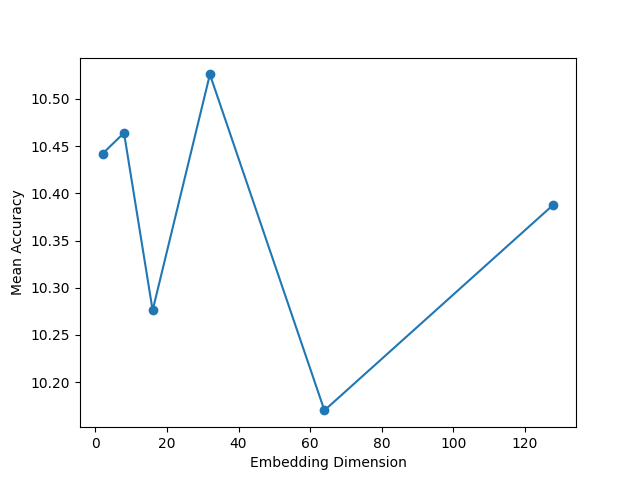
\includegraphics[width=0.9\textwidth,]{./Images/MNIST_VAE_sampling.png}
        \caption{Posterior Sampling}
    \end{subfigure}
    \begin{subfigure}[b]{0.4\textwidth}
        \centering
        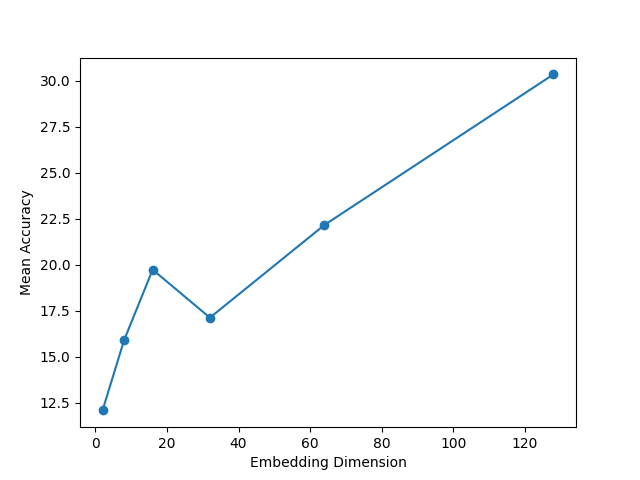
\includegraphics[width=0.9\textwidth]{./Images/MNIST_VAE_MAP.png}
        \caption{Maximum a posteriori}
    \end{subfigure}
    \caption{Classification Accuracy on MNIST Dataset for different latent sizes}
  \end{figure}
\end{frame}

\begin{frame}{\transparent{0.4} Towards \transparent{1}\textbf{Learning} \transparent{0.4}Better and Flexible \transparent{1}\textbf{Representations from Variational Autoencoders} \vspace{0.3em}}
  \begin{enumerate}
    \setcounter{enumi}{1}
    \item FashionMNIST Dataset
  \end{enumerate}
  \begin{itemize}
    \item Similar to MNIST Dataset, the classification accuracy for posterior sampling varies around 10 which is comparable to random labeling.
    % \item For Maximum a posteriori, the classification accuracy increases as we increase the dimensionality of the latent space.
  \end{itemize}
  \begin{figure}
    \begin{subfigure}[b]{0.4\textwidth}
        \centering
        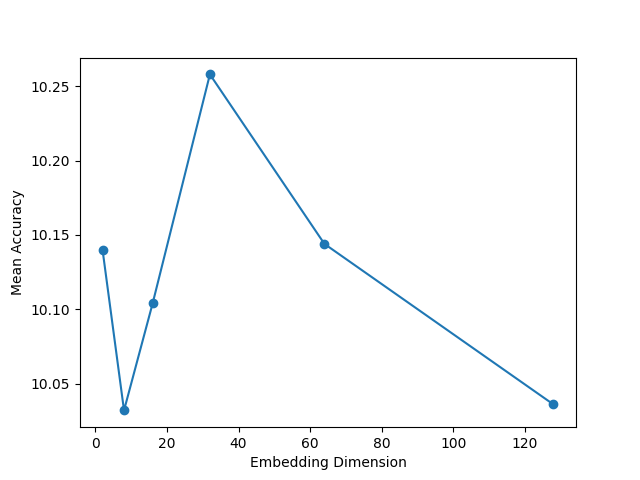
\includegraphics[width=0.9\textwidth,]{./Images/FashionMNIST_VAE_sampling.png}
        \caption{Posterior Sampling}
    \end{subfigure}
    % \begin{subfigure}[b]{0.4\textwidth}
    %     \centering
    %     \includegraphics[width=0.9\textwidth]{./Images/VAE_MAP.png}
    %     \caption{Maximum a posteriori}
    % \end{subfigure}
  \end{figure}
\end{frame}

\subsection{Shortcomings of VAEs}

\begin{frame}{\transparent{0.4} Towards \transparent{1}\textbf{Learning} \transparent{0.4}Better and Flexible \transparent{1}\textbf{Representations from Variational Autoencoders} \vspace{0.3em}}
  \begin{itemize}
    \item In order to understand why the classification accuracy was so low, we plotted the latent space representations.
    \item It was observed that input data belonging to the different classes have similar representations in latent space.
  \end{itemize}
  \begin{figure}
    \captionsetup{justification=centering}
    \begin{subfigure}[b]{0.4\textwidth}
        \centering
        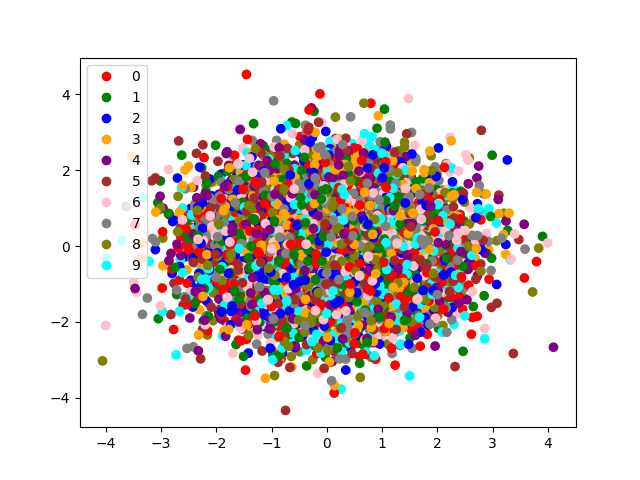
\includegraphics[width=\textwidth,]{./Images/latent_MNIST_VAE_Sampling.png}
        \caption{MNIST Dataset}
    \end{subfigure}
    \begin{subfigure}[b]{0.4\textwidth}
        \centering
        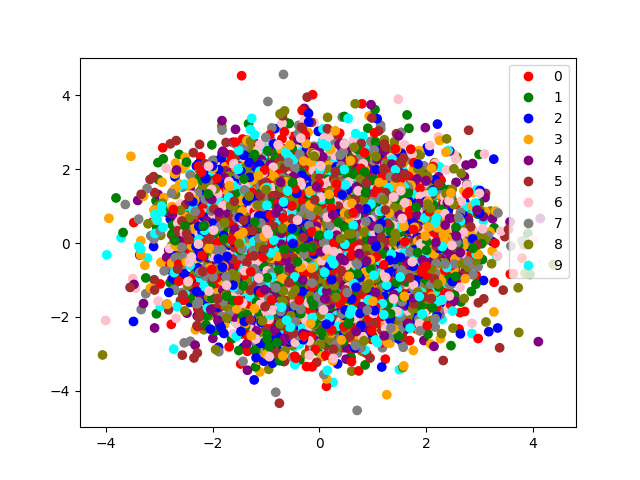
\includegraphics[width=\textwidth]{./Images/latent_FashionMNIST_VAE_Sampling.png}
        \caption{FashionMNIST Dataset}
    \end{subfigure}
    \caption{Latent Space for Posterior Sampling}
  \end{figure}
\end{frame}

\begin{frame}{\transparent{0.4} Towards \transparent{1}\textbf{Learning} \transparent{0.4}Better and Flexible \transparent{1}\textbf{Representations from Variational Autoencoders} \vspace{0.3em}}
  \begin{itemize}
    \item Due to similar representations, the classifier wasn't able to distinguish between two classes thus leading to poor classification.
    \item For higher dimensional latent representations, we used Principal Component Analysis (PCA) to project down the representations to 2-dimensional space for plotting the latent space.
  \end{itemize}
  \begin{figure}
    \captionsetup{justification=centering}
    \begin{subfigure}[b]{0.4\textwidth}
        \centering
        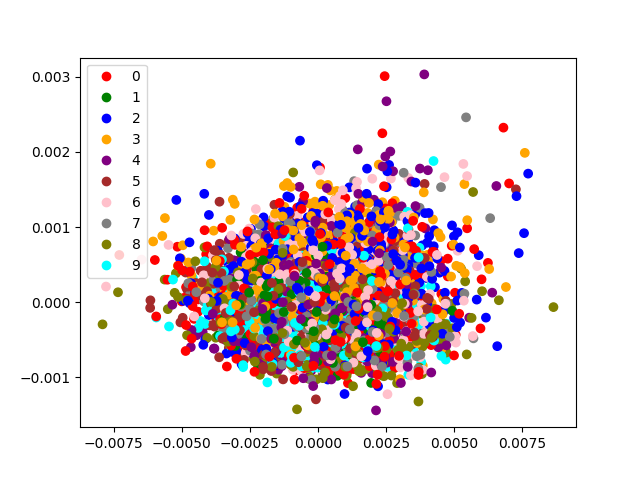
\includegraphics[width=\textwidth,]{./Images/latent_MNIST_VAE_MAP.png}
        \caption{MNIST Dataset}
    \end{subfigure}
    % \begin{subfigure}[b]{0.4\textwidth}
    %     \centering
    %     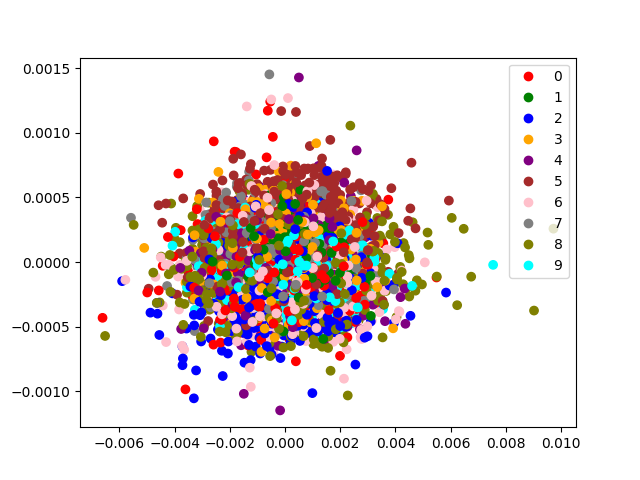
\includegraphics[width=\textwidth]{./Images/latent_FashionMNIST_VAE_MAP.png}
    %     \caption{FashionMNIST Dataset}
    % \end{subfigure}
    \caption{Latent Space for Maximum a posteriori}
  \end{figure}
\end{frame}

\section{InfoVAE}
\subsection{Intro to InfoVAE}

\begin{frame}{\transparent{0.4} Towards \transparent{1}\textbf{Learning Better} \transparent{0.4}and Flexible \transparent{1}\textbf{Representations from Variational Autoencoders} \vspace{0.3em}}
  \begin{itemize}
    \item Our next objective was to improve these latent space representations for better performance in downstream classification task.
    \item For this, we referred to \href{https://arxiv.org/pdf/1706.02262.pdf}{Zhao et. al., 2017} which proposed a new family of VAEs called InfoVAE.
    \item The paper discusses about two major problems of VAE :- 
    \begin{enumerate}
      \item The approximate inference distribution is often significantly different from the true posterior.
      \item When the conditional distribution is sufficiently expressive, the latent variables are often ignored.
    \end{enumerate}
    \item The paper argues that the above two problems arise due to ELBO objective used to train VAEs and proposes a new loss function.
    \item The following \href{https://ermongroup.github.io/blog/a-tutorial-on-mmd-variational-autoencoders/}{tutorial} serves as a good start for understanding InfoVAE. 
  \end{itemize}
\end{frame}

\subsection{Maximum Mean Discrepancy}

\begin{frame}{\transparent{0.4} Towards \transparent{1}\textbf{Learning Better} \transparent{0.4}and Flexible \transparent{1}\textbf{Representations from Variational Autoencoders} \vspace{0.3em}}
  \begin{itemize}
    \item In particular, we used Maximum Mean Discrepancy (MMD) instead of KL Divergence to quantify the distance between two distributions.
    \item Maximum Mean Discrepancy can be efficiently implemented using the kernel trick. Let $k(.\,,\,.)$ be any positive definite kernel then,
    \begin{align*}
      \mathcal{L}_{\text{MMD}}(q \,||\, p) &= \mathbb{E}_{p(z),\,p(z')}[k(z,\,z')] \\
                                           &+ \mathbb{E}_{q(z),\,q(z')}[k(z,\,z')] \\ 
                                           &- 2\mathbb{E}_{q(z),\,p(z')}[k(z,\,z')]
    \end{align*}
    \item In our project, we utilized Gaussian Kernel with $\sigma=1$ to implement Maximum Mean Discrepancy.
    \begin{align*}
      k(z,\,z') = e^{-\,\dfrac{||\,z-z'\,||^2}{2\sigma^2}}
    \end{align*}
  \end{itemize}
\end{frame}

\subsection{Implementation Details}

\begin{frame}{\transparent{0.4} Towards \transparent{1}\textbf{Learning Better} \transparent{0.4}and Flexible \transparent{1}\textbf{Representations from Variational Autoencoders} \vspace{0.3em}}
  \begin{itemize}
    \item For computing the MMD distance, we first simply generated $n$ samples from the prior distribution $p(z)$ and compared these generated samples with the encoder output.
    \item For training InfoVAE, we used the same hyperparameters as that of standard VAE. The additional hyperparameter $n$ was set to 200.
    \item We also implemented an early stopping module to prevent overfitting and employed 5-fold cross validation for evaluation.
    \item We used the following Github \href{https://github.com/napsternxg/pytorch-practice}{repository} for reference while implementing our model.
  \end{itemize}
\end{frame}

\subsection{Results}

\begin{frame}{\transparent{0.4} Towards \transparent{1}\textbf{Learning Better} \transparent{0.4}and Flexible \transparent{1}\textbf{Representations from Variational Autoencoders} \vspace{0.3em}}
  \begin{enumerate}
    \item MNIST Dataset
  \end{enumerate}
  \begin{itemize}
    \item Barring the 2-dimensional case, the classification accuracy for posterior sampling approaches 98\% which is comparable to SOTA.
    % \item For Maximum a posteriori, the classification accuracy increases as we increase the dimensionality of the latent space.
  \end{itemize}
  \begin{figure}
    \begin{subfigure}[b]{0.45\textwidth}
        \centering
        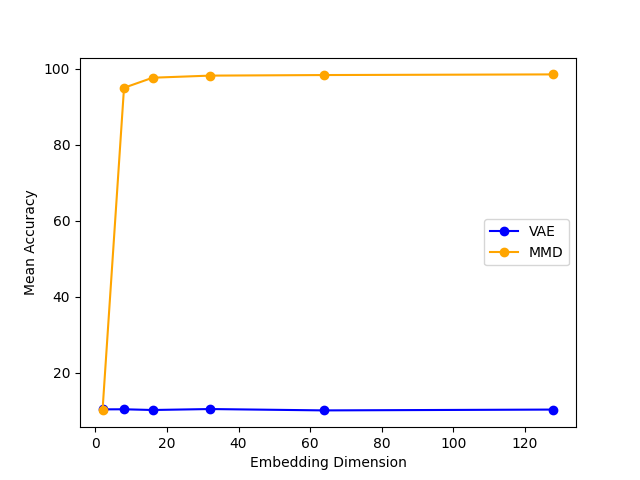
\includegraphics[width=0.9\textwidth,]{./Images/MNIST_Compare_Sampling.png}
        \caption{Posterior Sampling}
    \end{subfigure}
    % \begin{subfigure}[b]{0.4\textwidth}
    %     \centering
    %     \includegraphics[width=0.9\textwidth]{./Images/VAE_MAP.png}
    %     \caption{Maximum a posteriori}
    % \end{subfigure}
  \end{figure}
\end{frame}

\begin{frame}{\transparent{0.4} Towards \transparent{1}\textbf{Learning Better} \transparent{0.4}and Flexible \transparent{1}\textbf{Representations from Variational Autoencoders} \vspace{0.3em}}
  \begin{enumerate}
    \setcounter{enumi}{1}
    \item FashionMNIST Dataset
  \end{enumerate}
  \begin{itemize}
    \item Similar to MNIST Dataset, classification accuracy for posterior sampling approaches 90\%.
  % \item For Maximum a posteriori, the classification accuracy increases as we increase the dimensionality of the latent space.
  \end{itemize}
  \begin{figure}
    \begin{subfigure}[b]{0.4\textwidth}
        \centering
        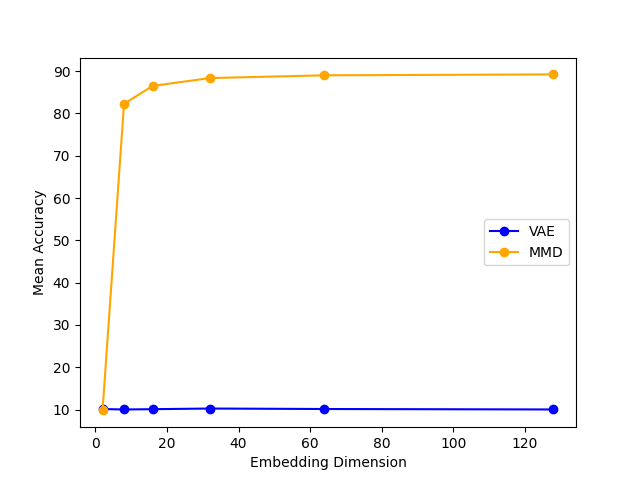
\includegraphics[width=0.9\textwidth,]{./Images/FashionMNIST_MMD_sampling.png}
        \caption{Posterior Sampling}
    \end{subfigure}
    % \begin{subfigure}[b]{0.4\textwidth}
    %     \centering
    %     \includegraphics[width=0.9\textwidth]{./Images/VAE_MAP.png}
    %     \caption{Maximum a posteriori}
    % \end{subfigure}
  \end{figure}
\end{frame}

\begin{frame}{\transparent{0.4} Towards \transparent{1}\textbf{Learning Better} \transparent{0.4}and Flexible \transparent{1}\textbf{Representations from Variational Autoencoders} \vspace{0.3em}}
  \begin{itemize}
    \item After plotting the latent space
  % \item For Maximum a posteriori, the classification accuracy increases as we increase the dimensionality of the latent space.
  \end{itemize}
  % \begin{figure}
  %   \begin{subfigure}[b]{0.4\textwidth}
  %       \centering
  %       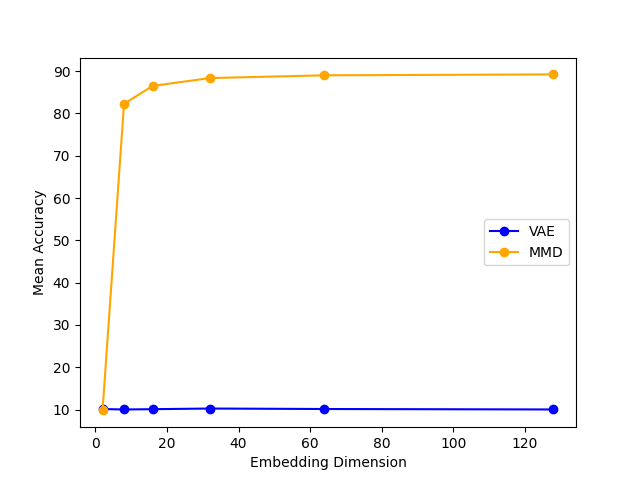
\includegraphics[width=0.9\textwidth,]{./Images/FashionMNIST_MMD_sampling.png}
  %       \caption{Posterior Sampling}
  %   \end{subfigure}
    % \begin{subfigure}[b]{0.4\textwidth}
    %     \centering
    %     \includegraphics[width=0.9\textwidth]{./Images/VAE_MAP.png}
    %     \caption{Maximum a posteriori}
    % \end{subfigure}
  % \end{figure}
\end{frame}

\section{Flexible Representations}

\begin{frame}{\transparent{0.4} Towards Learning Better and \transparent{1}\textbf{Flexible Representations} \transparent{0.4}from Variational Autoencoders \vspace{0.3em}}
  \begin{itemize}
    \item So far, we utilized InfoVAE to improve the representations learnt from Variational Autoencoder architecture.
    \item However, when training these representations, we didn't consider the computational and statistical constraints of the downstream task.
    \item In practice, these representations would be shared with different clients with varying computational resources. 
    \item In this context, rigid fixed-capacity representations can be either over or under-accommodating to the task at hand.
  \end{itemize}
\end{frame}

\subsection{Matryoshka Representation Learning}

\begin{frame}{\transparent{0.4} Towards Learning Better and \transparent{1}\textbf{Flexible Representations} \transparent{0.4}from Variational Autoencoders \vspace{0.3em}}
  \begin{itemize}
    \item Our objective in the latter half of the project would be to make the representations learnt from VAEs flexible.
    \item In order to achieve this goal, we refer to \href{https://proceedings.neurips.cc/paper_files/paper/2022/file/c32319f4868da7613d78af9993100e42-Paper-Conference.pdf}{Kusupati et al., 2022} which proposes \textbf{Matryokshka Representation Learning}.
  \end{itemize}
  \pause
  \begin{center}
    \begin{figure}
      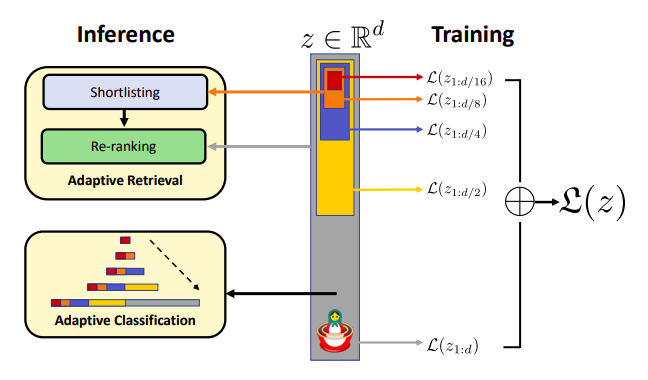
\includegraphics[width=0.6\textwidth]{./Images/mrl.png}
      \caption{Matryoshka Representation Learning}
    \end{figure}
  \end{center}
\end{frame}

\begin{frame}{\transparent{0.4} Towards Learning Better and \transparent{1}\textbf{Flexible Representations} \transparent{0.4}from Variational Autoencoders \vspace{0.3em}}
  \begin{itemize}
    \item The paper argues that gradient-based training of deep learning models tends to diffuse information across the entire representation vector leading to rigidity.
    \item To induce flexibility in the learned representation, Matryoshka Representation Learning encodes information at different granularities 
    \item In this way, a single embedding can adapt to the computational constraints of multiple downstream tasks.
    \item There have been several applications of Matryoshka Representation Learning :-
    \begin{enumerate}
      \item MatFormer (\href{https://arxiv.org/pdf/2310.07707.pdf}{Kudugunta, Sneha, et al., 2023})
      \item AdANNS (\href{https://proceedings.neurips.cc/paper_files/paper/2023/file/f062da1973ac9ac61fc6d44dd7fa309f-Paper-Conference.pdf}{Rege, Aniket, et al., 2024})
    \end{enumerate}
    \item In this project, we intend to implement Matryokshka Representation Learning in the VAE algorithm in order to obtain flexible latent representations.
  \end{itemize}
\end{frame}

\section{Future Roadmap}

\begin{frame}{Future Roadmap}
  \begin{enumerate}
    \item Implement \href{https://proceedings.neurips.cc/paper_files/paper/2022/file/c32319f4868da7613d78af9993100e42-Paper-Conference.pdf}{Kusupati et al., 2022} paper.
    \begin{itemize}
      \item Particularly, we explore the application of MRL in downstream classification task.
      \item We will use Resnet-50 models and ImageNet-1K dataset for evaluating this task.
    \end{itemize} 
    \item We integrate Matryokshka Representation Learning in VAE algorithm.
    \item Compare the results of MRL with individually trained models.
  \end{enumerate}
\end{frame}

\end{document}